\section*{Figures}
	 
	
	\begin{figure}[h!]
		\label{fig:transmitpower}
		\caption{\csentence{Sample Power Interpolation}
		Here an power interpolation was done for 20 cell sites with a random transmitter power in the range of 45--52dBm}
		\includegraphics[width=0.9\columnwidth]{senderpower}
	\end{figure}
	\begin{figure}[h!]
		\label{fig:populationgrid}
		\caption{\csentence{Popualtion grid} The following demonstrates an area with 3 different population densities. Our assumption is that people will more likely start or end their journey in a higher populated area.
		}
		\includegraphics[width=0.9\columnwidth]{populationgrid}
	\end{figure}
	\begin{figure}[h!]
		\label{fig:handover}
		\caption{\csentence{Types of handover} An overlapping handover (a) and an unconnected handover are depicted together with the estimated handover position (red point)
		}
		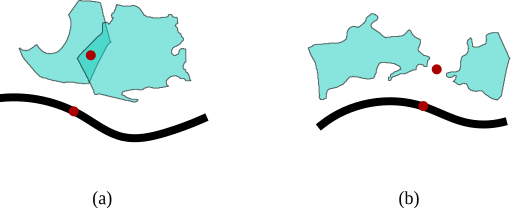
\includegraphics[width=0.9\columnwidth]{handover}
	\end{figure}
	
	\begin{figure*}[h!]
		\label{fig:563}
		\caption{\csentence{Trajectoy 1} A comparison of handover deviations between the real handover position and the estimated one with the three coverage estimation methods (P coverage prediction, PB coverage prediction with buildings and V Voronoi)
		}
		\includegraphics[height=0.40\textheight]{images/563standalone.png}
	\end{figure*}
	
	
	
	\begin{figure*}[h!]
		\label{fig:144}
		\caption{\csentence{Trajectory 4} A comparison of handover deviations between the real handover position and the estimated one with the three coverage estimation methods (P coverage prediction, PB coverage prediction with buildings and V Voronoi)
		}
		\includegraphics[height=0.40\textheight]{images/144standalone.png}
	\end{figure*}
	
	
	\begin{figure}[h!]
		\label{fig:handoverdeviation}
		\caption{\csentence{Trajectory 1 handover deviations} A comparison of handover deviations between the real handover position and the estimated one with the three coverage estimation methods (P coverage prediction, PB coverage prediction with buildings and V Voronoi)
		}
		\includegraphics[width=0.9\columnwidth]{images/563_HandoverDeviation}
	\end{figure}
	
	
	\begin{figure}[h!]
		\label{fig:velocity}
		\caption{\csentence{Trajectory 1 velocity without adaption} The estimated velocity for all three coverage estimation methods (P coverage prediction, PB coverage prediction with buildings and V Voronoi) without the adaption algorithm
		}
		\includegraphics[width=0.9\columnwidth]{images/563_SpeedWithoutAdaption}
	\end{figure}
	
	\begin{figure}[h!]
		\label{fig:velocityadaption}
		\caption{\csentence{Trajectory 1 Velocity with adaption} The estimated velocity for all three coverage estimation methods (P coverage prediction, PB coverage prediction with buildings and V Voronoi) with the adaption algorithm
		}
		\includegraphics[width=0.9\columnwidth]{images/563_SpeedsWithAdaption}
	\end{figure}
	%%%%%%%%%%%%%%%%%%%%%%%%%%%%%%%%%%%
	%%                               %%
	%% Tables                        %%
	%%                               %%
	%%%%%%%%%%%%%%%%%%%%%%%%%%%%%%%%%%%
	
	%% Use of \listoftables is discouraged.
	%%
	\section*{Tables}
	%\begin{table}[h!]
	%\caption{The phone state captured by the Android application}
	%\begin{tabular}{|c|c|c|c|c|c|c|}
	%\hline
	%\textbf{Time stamp} & \textbf{Id} & \textbf{Cell-Id} & \textbf{LAC} &\textbf{State} & \textbf{Longitude} & \textbf{Latitude} \\ \hline
	%1327678833 & 4 & 51520 & 5501 & 0 & 48.36632 & 14.51978 \\
	%1327678834 & 4 & 51510 & 5501 & 2 & 48.36606 & 14.52017 \\
	%1327678835 & 4 & 51510 & 5501 & 2 & 48.36591 & 14.52035 \\
	%1327678836 & 4 & 51510 & 5501 & 2 & 48.36583 & 14.52046 \\
	%1327678837 & 4 & 51510 & 5501 & 2 & 48.36573 & 14.52061
	%\\ \hline
	%\end{tabular}
	%\label{table:phonestate}
	%\end{table}
	
	
	
	\begin{table}[h]
		\caption{Overview of the start and end position and the amount of handover events (unfiltered handover) for the four test drive trajectories}
		\begin{tabular}{|c|c|c|c|}
			\hline
			\textbf{$\#$} & \textbf{Start [Lat,Lon]} & \textbf{End [Lat,Lon]} & \textbf{Handover} \\ \hline
			1             & 48.28105,14.30415        & 48.33499,14.3780       & 18 (22)           \\ %563
			2             & 48.31616,14.29052        & 48.28169,14.30275      & 17 (19)           \\  %1058
			3             & 48.13993,16.32367        & 48.19880,16.25597      & 16 (20)           \\ %367
			4             & 48.19283,16.27260        & 48.15278,16.30172      & 27 (37)           \\  \hline %144
		\end{tabular}
		\label{table:tracks}
	\end{table}
	
	
	\begin{table}[h]
		\caption{The route similarity computed with the discrete Hausdorff distance and the Fr\'{e}chet distance}
		\begin{tabular}{|c|c|c|}
			\hline
			\textbf{Trajectory} & \textbf{$d_{H}(X,Y)$ } & \textbf{$\delta_F(f,g)$} \\ \hline
			1                   & $0.0135^\circ$         & $0.0047^\circ$           \\ %563
			2                   & $0.0075^\circ$         & $0.0015^\circ$           \\  %1058
			3                   & $0.0151^\circ$         & $0.0021^\circ$           \\ %367
			4                   & $0.0107^\circ$         & $0.0012^\circ$           \\  \hline %144
		\end{tabular}
		\label{table:routesim}
	\end{table}
	
	%\begin{table}[h]
	%\sisetup{round-mode=places,round-precision=3,tight-spacing=true}% hier ggf. anpassen! (siehe siunitx-Anleitung)
	%
	%\caption{The min, first quartile, median, mean, third quartile and max handover position deviation in \si{\km} for each of the four trajectories for the three different coverage predictions M (P coverage prediction, PB coverage prediction with buildings and V Voronoi)}
	%\begin{tabular}{|c|c|S|S|S|S|S|S|}
	%\hline
	%\textbf{$\#$} & \textbf{M}& \multicolumn{1}{c|}{\bfseries$\min$}& \multicolumn{1}{c|}{\textbf{$Q_1$}  }    & \multicolumn{1}{c|}{\textbf{$\tilde{x}$} }& \multicolumn{1}{c|}{\textbf{$\bar{x}$} }   & \multicolumn{1}{c|}{\textbf{$Q_3$}}    & \multicolumn{1}{c|}{\textbf{$\max$}}   \\ \hline
	%1 & P  & 0.1610&  0.4680  & 0.6630&  0.7049 & 0.8780 & 1.4030  \\  \hline %563
	%1&  PB  & 0.1010 &  0.5470 &  0.7160 &  0.7109  & 0.9280 & 1.3150  \\  \hline  %1058
	%1 &  V  & 0.1420 & 0.4200 & 0.8370 & 0.7148 & 1.0230 & 1.1550 \\  \hline%367
	%2 & P   & 0.2190 &  0.2860 & 0.3205&  0.4013&  0.4830 & 0.9000\\ \hline %563
	%2&  PB   & 0.1320 & 0.2605 & 0.3455&  0.3993 & 0.5245&  0.8840   \\   \hline%1058
	%2 &  V  & 0.0480 & 0.2290 &  0.3430 &  0.3861  & 0.4815  & 0.9000   \\  \hline %367
	%3 & P   & 0.1110 &  0.3595 & 0.4490 &  0.6769  & 0.6040 & 3.7860   \\   \hline%563
	%3&  PB  & 0.1480 & 0.3375  & 0.4510 &  0.6789 & 0.5355  & 4.0620   \\   \hline%1058
	%3 &  V  & 0.0130 &  0.2805  & 0.4090  & 0.6689 & 0.6385 &  4.0850   \\  \hline%367
	%4 & P &  0.0200 &  0.2230 & 0.3090 &  0.3552 & 0.5040  & 0.8630  \\  \hline%563
	%4&  PB   & 0.0300 &  0.2133 & 0.3245  & 0.3588 & 0.5060 &  0.8500  \\   \hline%1058
	%4 &  V& 0.0100 &  0.1748 &  0.3210 &  0.3275 & 0.4428 & 0.8020  \\  \hline %144
	%\end{tabular}
	%\label{table:handover}
	%\end{table}
	
	\begin{table}[h]
		\caption{The min, first quartile, median, mean, third quartile and max handover position deviation in kilometer for each of the four trajectories for the three different coverage predictions M (P coverage prediction, PB coverage prediction with buildings and V Voronoi)}
		\begin{tabular}{|c|c|c|c|c|c|c|c|}
			\hline
			\textbf{$\#$} & \textbf{M} & \textbf{$\min$} & \textbf{$Q_1$} & \textbf{$\tilde{x}$} & \textbf{$\bar{x}$} & \textbf{$Q_3$} & \textbf{$\max$} \\ \hline
			1             & P          & 0.161           & 0.468          & 0.663                & 0.705              & 0.878          & 1.403           \\ \hline
			1             & PB         & 0.101           & 0.547          & 0.716                & 0.711              & 0.928          & 1.315           \\ \hline
			1             & V          & 0.142           & 0.420          & 0.837                & 0.715              & 1.023          & 1.155           \\ \hline
			2             & P          & 0.219           & 0.286          & 0.321                & 0.401              & 0.483          & 0.900           \\ \hline
			2             & PB         & 0.132           & 0.261          & 0.346                & 0.399              & 0.525          & 0.884           \\ \hline
			2             & V          & 0.048           & 0.229          & 0.343                & 0.386              & 0.482          & 0.900           \\ \hline
			3             & P          & 0.111           & 0.360          & 0.449                & 0.677              & 0.604          & 3.786           \\ \hline
			3             & PB         & 0.148           & 0.338          & 0.451                & 0.679              & 0.536          & 4.062           \\ \hline
			3             & V          & 0.013           & 0.281          & 0.409                & 0.669              & 0.639          & 4.085           \\ \hline
			4             & P          & 0.020           & 0.223          & 0.309                & 0.355              & 0.504          & 0.863           \\ \hline
			4             & PB         & 0.030           & 0.213          & 0.325                & 0.359              & 0.506          & 0.850           \\ \hline
			4             & V          & 0.010           & 0.175          & 0.321                & 0.328              & 0.443          & 0.802           \\ \hline
		\end{tabular}
		\label{table:handover}
	\end{table}
	
	
	\begin{table}[h]
		\caption{The MAE and RMSE for each of the four trajectories for the three different coverage predictions}
		\begin{tabular}{|c|c|c|c|c|c|}
			\hline
			\textbf{$\#$} & \textbf{M} & \textbf{MAE} & \textbf{RMSE} & \textbf{adaptMAE} & \textbf{adaptRMSE} \\ \hline
			1             & P          & 42.365       & 62.593        & 23.360            & 31.514             \\  \hline %563
			1             & PB         & 50.315       & 69.985        & 23.127            & 29.142             \\  \hline  %1058
			1             & V          & 59.704       & 85.549        & 17.648            & 25.250             \\  \hline%367
			2             & P          & 81.304       & 138.707       & 8.970             & 16.047             \\ \hline %563
			2             & PB         & 60.964       & 99.090        & 9.436             & 12.086             \\   \hline%1058
			2             & V          & 113.999      & 181.854       & 13.029            & 16.932             \\  \hline %367
			3             & P          & 21.125       & 26.808        & 13.305            & 17.799             \\   \hline%563
			3             & PB         & 26.384       & 33.786        & 11.941            & 16.607             \\   \hline%1058
			3             & V          & 28.449       & 40.088        & 13.036            & 18.781             \\  \hline%367
			4             & P          & 58.425       & 150.199       & 17.081            & 22.000             \\  \hline%563
			4             & PB         & 48.061       & 125.747       & 14.553            & 17.795             \\   \hline%1058
			4             & V          & 72.715       & 191.037       & 15.388            & 21.599             \\  \hline %144
		\end{tabular}
		\label{table:results}
	\end{table}